% 大学物理实验报告

\documentclass[UTF8]{ctexart}

\usepackage{amsmath}        %数学公式
\usepackage{cases}          %联立编号
\usepackage{cite}           %引用

\usepackage{graphicx}       %插入图片
\usepackage{float}          %设置图片浮动位置
\usepackage{subfigure}      %插入多图时用子图显示

\usepackage{anyfontsize}    %解决一个奇怪的字体大小报错问题
\usepackage{fancyhdr}       %页眉、页脚、页码
\usepackage[a4paper, margin=1in]{geometry}    %纸张大小


\setlength{\headheight}{16pt}
\pagestyle{fancy}
\fancyhf{}


\title{高温超导材料转变温度测定实验报告}
\author{\LaTeX\ by\ Jerry\ }
\date{\today}
\pagenumbering{arabic}

\begin{document}

\fancyhead[L]{Jerry}
\fancyhead[C]{高温超导材料转变温度测定实验}
\fancyfoot[C]{\thepage}

\maketitle
\tableofcontents
\newpage

\section{原始数据}

    \subsection{超导样品电阻测量}

    1. 数字万用表两条外引线电阻测量:$R_{outwire}=0.10\Omega$

    2. 超导盒内样品与内在引线、外表引线串联电阻之和:$R_{sum}=0.50\Omega$

    3. 超导盒内样品与内在引线电阻值:$R_{wire}+R_{SC}=0.40\Omega$

    4. CH3工作模式:恒压或恒流:恒流,输出电压$V=643$mV,输出电流$I=1000$mA,
    总负载电阻$R=0.643$m$\Omega$,$R_{SC}=0.413$m$\Omega$

    \subsection{用电流换向法消除乱真电势的影响}

    $V_{Meas1}$(3档)$=0.414$mV,$V_{Meas2}$(4档)$=-0.416$mV,$V$乱真电势$=1\mu$V

    (与超导样品上的电压相比,乱真电势很小,而且会随温度变化而改变,由于实验过程中换向开关不易频繁操作,
    同学们测出室温下的乱真电势和超导态下的乱真电势即可)

    \subsection{用铂电阻温度计测量温度}

    1. 限流电阻$R_0=10$k$\Omega$

    2. 计算四位半数字电压表的显示初值$V_{calc}=109.70$mV,(室温:24.9$^{\circ}$C,$R_{Pt}=109.70\Omega$)

    3. 实际四位半电压表数值$V_{real}=108.78$mV,

    4. CH1工作模式:恒压或恒流:恒压,输出电压$V=10.003$V,输出电流$I=1$mA

    \subsection{用电磁感应法测超导样品对感应电压的影响}

    正弦信号$f=700$Hz,直流偏置offset=0,$V_{pp}=2.00$V,$V_{induction}=10.62$mV

    \subsection{降温实验}

    \subsubsection{降温}

    1. 降温数据:(注意:样品电压突降至0微伏的极小值并稳定不变后,继续每隔0.5分钟测一次,共5组左右)

    \begin{table}[H]
        \centering
        \begin{tabular}{|l|l|l|l|l|l|l|l|l|l|l|}
        \hline
            $V_{Pt}$(mV) & 107.75 & 103.84 & 99.95 & 95.97 & 92.10 & 88.20 & 84.24 & 80.27 & 76.35 & 72.38 \\ \hline
            $V_{Sample}$($\mu$V) & 413 & 409 & 404 & 397 & 387 & 378 & 369 & 359 & 327 & 311 \\ \hline
            $V_B$(mV) & 10.63 & 10.60 & 10.60 & 10.64 & 10.61 & 10.60 & 10.64 & 10.69 & 10.74 & 10.87 \\ \hline
            \hline
            $V_{Pt}$(mV) & 68.38 & 64.36 & 60.34 & 56.28 & 52.25 & 48.22 & 44.15 & 40.07 & 35.96 & 31.80 \\ \hline
            $V_{Sample}$($\mu$V) & 296 & 281 & 264 & 250 & 233 & 215 & 197 & 178 & 158 & 140 \\ \hline
            $V_B$(mV) & 11.01 & 11.15 & 11.24 & 11.43 & 11.60 & 11.72 & 11.80 & 11.89 & 11.99 & 12.13 \\ \hline
            \hline
            $V_{Pt}$(mV) & 29.74 & 29.46 & 29.06 & 28.62 & 28.19 & 27.79 & 27.41 & 25.60 & 24.38 & 23.64 \\ \hline
            $V_{Sample}$($\mu$V) & 129 & 94 & 21 & 4 & 2 & 2 & 1 & 1 & 2 & 2 \\ \hline
            $V_B$(mV) & 12.16 & 12.18 & 12.06 & 11.41 & 11.10 & 10.97 & 10.87 & 10.69 & 10.66 & 10.66 \\ \hline
        \end{tabular}
        \caption{降温时电压记录表格} %最终文档中希望显示的图片标题
        \label{降温原数据表格} %用于文内引用的标签
    \end{table}

    超导态下:$V_{Meas1}$(3档)=0.001mV,$V_{Meas2}$(4档)=0.002mV,$V$乱真电势=1.5$\mu$V,
    简化起见,乱真电势修正统一以此值为准 。

    \subsubsection{升温}

    \begin{table}[H]
        \centering
        \begin{tabular}{|l|l|l|l|l|l|l|l|l|l|l|}
        \hline
            $V_{Pt}$(mV) & 23.65 & 25.71 & 27.76 & 29.84 & 31.85 & 33.94 & 34.76 & 35.15 & 35.61 & 36.00 \\ \hline
            $V_{Sample}$($\mu$V) & 2 & 2 & 3 & 3 & 2 & 3 & 2 & 3 & 3 & 5 \\ \hline
            $V_B$(mV) & 10.70 & 10.69 & 10.70 & 10.73 & 10.76 & 10.91 & 11.06 & 11.16 & 11.37 & 11.62 \\ \hline
            \hline
            $V_{Pt}$(mV) & 36.38 & 36.79 & 37.20 & 37.64 & 38.04 & 38.44 & 38.84 & 39.27 & 39.65 & 40.08 \\ \hline
            $V_{Sample}$($\mu$V) & 15 & 57 & 121 & 131 & 132 & 134 & 135 & 137 & 139 & 140 \\ \hline
            $V_B$(mV) & 12.04 & 12.21 & 12.21 & 12.20 & 12.19 & 12.19 & 12.17 & 12.17 & 12.16 & 12.16 \\ \hline
            \hline
            $V_{Pt}$(mV) & 40.49 & 40.90 & 41.32 & 41.72 & 42.12 & 42.54 & 42.93 & 43.34 & 43.72 & 44.13 \\ \hline
            $V_{Sample}$($\mu$V) & 141 & 142 & 143 & 146 & 147 & 148 & 150 & 151 & 153 & 154 \\ \hline
            $V_B$(mV) & 12.15 & 12.14 & 12.13 & 12.12 & 12.12 & 12.11 & 12.10 & 12.09 & 12.09 & 12.08 \\ \hline
        \end{tabular}
        \caption{升温时电压记录表格} %最终文档中希望显示的图片标题
        \label{升温原数据表格} %用于文内引用的标签
    \end{table}

\section{数据处理}

    \subsection{计算样品温度}

    用测得的铂电阻电压数据,计算样品温度$t$

    计算样品电阻$R_t$和乱真电势。比较乱真电势与超导转变后的样品电压的数量级大小。

    \subsubsection{降温}

    \begin{table}[H]
        \centering
        \begin{tabular}{|l|l|l|l|l|l|l|l|l|l|l|}
        \hline
            $V_{Pt}$(mV) & 107.75 & 103.84 & 99.95 & 95.97 & 92.10 & 88.20 & 84.24 & 80.27 & 76.35 & 72.38 \\ \hline
            $R_{Pt}(\Omega)$ & 107.75 & 103.84 & 99.95 & 95.97 & 92.10 & 88.20 & 84.24 & 80.27 & 76.35 & 72.38 \\ \hline
            温度($^{\circ}$C) & 20 & 10 & 0 & -10 & -20 & -30 & -40 & -50 & -60 & -70 \\ \hline
            $V_{Sample}$($\mu$V) & 413 & 409 & 404 & 397 & 387 & 378 & 369 & 359 & 327 & 311 \\ \hline
            $R_{Sample}$(m$\Omega$) & 413 & 409 & 404 & 397 & 387 & 378 & 369 & 359 & 327 & 311 \\ \hline
            \hline
            $V_{Pt}$(mV) & 68.38 & 64.36 & 60.34 & 56.28 & 52.25 & 48.22 & 44.15 & 40.07 & 35.96 & 31.80 \\ \hline
            $R_{Pt}(\Omega)$ & 68.38 & 64.36 & 60.34 & 56.28 & 52.25 & 48.22 & 44.15 & 40.07 & 35.96 & 31.80 \\ \hline
            温度($^{\circ}$C) & -80 & -90 & -100 & -110 & -120 & -130 & -140 & -150 & -160 & -170 \\ \hline
            $V_{Sample}$($\mu$V) & 296 & 281 & 264 & 250 & 233 & 215 & 197 & 178 & 158 & 140 \\ \hline
            $R_{Sample}$(m$\Omega$) & 296 & 281 & 264 & 250 & 233 & 215 & 197 & 178 & 158 & 140 \\ \hline
            \hline
            $V_{Pt}$(mV) & 29.74 & 29.46 & 29.06 & 28.62 & 28.19 & 27.79 & 27.41 & 25.60 & 24.38 & 23.64 \\ \hline
            $R_{Pt}(\Omega)$ & 29.74 & 29.46 & 29.06 & 28.62 & 28.19 & 27.79 & 27.41 & 25.60 & 24.38 & 23.64 \\ \hline
            温度($^{\circ}$C) & -175 & -176 & -177 & -178 & -179 & -180 & -181 & -185 & -188 & -190 \\ \hline
            $V_{Sample}$($\mu$V) & 129 & 94 & 21 & 4 & 2 & 2 & 1 & 1 & 2 & 2 \\ \hline
            $R_{Sample}$(m$\Omega$) & 129 & 94 & 21 & 4 & 2 & 2 & 1 & 1 & 2 & 2 \\ \hline
        \end{tabular}
        \caption{降温时计算$Pt$的电阻、温度、与样品的电阻} %最终文档中希望显示的图片标题
        \label{降温计算表格} %用于文内引用的标签
    \end{table}

    \subsubsection{升温}

    \begin{table}[H]
        \centering
        \begin{tabular}{|l|l|l|l|l|l|l|l|l|l|l|}
        \hline
            $V_{Pt}$(mV) & 23.65 & 25.71 & 27.76 & 29.84 & 31.85 & 33.94 & 34.76 & 35.15 & 35.61 & 36.00 \\ \hline
            $R_{Pt}(\Omega)$ & 23.65 & 25.71 & 27.76 & 29.84 & 31.85 & 33.94 & 34.76 & 35.15 & 35.61 & 36.00 \\ \hline
            温度($^{\circ}$C) & -190 & -185 & -180 & -175 & -170 & -165 & -163 & -162 & -161 & -160 \\ \hline
            $V_{Sample}$($\mu$V) & 2 & 2 & 3 & 3 & 2 & 3 & 2 & 3 & 3 & 5 \\ \hline
            $R_{Sample}$(m$\Omega$) & 2 & 2 & 3 & 3 & 2 & 3 & 2 & 3 & 3 & 5 \\ \hline
            \hline
            $V_{Pt}$(mV) & 36.38 & 36.79 & 37.20 & 37.64 & 38.04 & 38.44 & 38.84 & 39.27 & 39.65 & 40.08 \\ \hline
            $R_{Pt}(\Omega)$ & 36.38 & 36.79 & 37.20 & 37.64 & 38.04 & 38.44 & 38.84 & 39.27 & 39.65 & 40.08 \\ \hline
            温度($^{\circ}$C) & -159 & -158 & -157 & -156 & -155 & -154 & -153 & -152 & -151 & -150 \\ \hline
            $V_{Sample}$($\mu$V) & 15 & 57 & 121 & 131 & 132 & 134 & 135 & 137 & 139 & 140 \\ \hline
            $R_{Sample}$(m$\Omega$) & 15 & 57 & 121 & 131 & 132 & 134 & 135 & 137 & 139 & 140 \\ \hline
            \hline
            $V_{Pt}$(mV) & 40.49 & 40.90 & 41.32 & 41.72 & 42.12 & 42.54 & 42.93 & 43.34 & 43.72 & 44.13 \\ \hline
            $R_{Pt}(\Omega)$ & 40.49 & 40.90 & 41.32 & 41.72 & 42.12 & 42.54 & 42.93 & 43.34 & 43.72 & 44.13 \\ \hline
            温度($^{\circ}$C) & -149 & -148 & -147 & -146 & -145 & -144 & -143 & -142 & -141 & -140 \\ \hline
            $V_{Sample}$($\mu$V) & 141 & 142 & 143 & 146 & 147 & 148 & 150 & 151 & 153 & 154 \\ \hline
            $R_{Sample}$(m$\Omega$) & 141 & 142 & 143 & 146 & 147 & 148 & 150 & 151 & 153 & 154 \\ \hline
       \end{tabular}
        \caption{升温时计算$Pt$的电阻、温度、与样品的电阻} %最终文档中希望显示的图片标题
        \label{升温计算表格} %用于文内引用的标签
    \end{table}

    超导态下:$V_{Meas1}$(3档)=0.001mV,$V_{Meas2}$(4档)=0.002mV,故$V$乱真电势=1.5$\mu$V。
    可以看出乱真电势与超导转变后的样品电压在同一个数量级,乱真电势不可以被忽略不计。

    \subsection{做图}

    分别画出样品在降温、升温过程中的电阻—温度特性曲线和感应电压—温度曲线:

    \subsubsection{降温}

    \begin{table}[H]
        \centering
        \begin{tabular}{|l|l|l|l|l|l|l|l|l|l|l|}
        \hline
            温度($^{\circ}$C) & 20 & 10 & 0 & -10 & -20 & -30 & -40 & -50 & -60 & -70 \\ \hline
            $R_{Sample}$(m$\Omega$) & 413 & 409 & 404 & 397 & 387 & 378 & 369 & 359 & 327 & 311 \\ \hline
            $V_B$(mV) & 10.63 & 10.60 & 10.60 & 10.64 & 10.61 & 10.60 & 10.64 & 10.69 & 10.74 & 10.87 \\ \hline
            \hline
            温度($^{\circ}$C) & -80 & -90 & -100 & -110 & -120 & -130 & -140 & -150 & -160 & -170 \\ \hline
            $R_{Sample}$(m$\Omega$) & 296 & 281 & 264 & 250 & 233 & 215 & 197 & 178 & 158 & 140 \\ \hline
            $V_B$(mV) & 11.01 & 11.15 & 11.24 & 11.43 & 11.60 & 11.72 & 11.80 & 11.89 & 11.99 & 12.13 \\ \hline
            \hline
            温度($^{\circ}$C) & -175 & -176 & -177 & -178 & -179 & -180 & -181 & -185 & -188 & -190 \\ \hline
            $R_{Sample}$(m$\Omega$) & 129 & 94 & 21 & 4 & 2 & 2 & 1 & 1 & 2 & 2 \\ \hline
            $V_B$(mV) & 12.16 & 12.18 & 12.06 & 11.41 & 11.10 & 10.97 & 10.87 & 10.69 & 10.66 & 10.66 \\ \hline
        \end{tabular}
        \caption{降温做图表格} %最终文档中希望显示的图片标题
        \label{降温做图表格} %用于文内引用的标签
    \end{table}

    % \begin{figure}[H] %H为当前位置,!htb为忽略美学标准,htbp为浮动图形
    %     \begin{minipage}[t]{0.48\linewidth}
    %         \centering %图片居中
    %         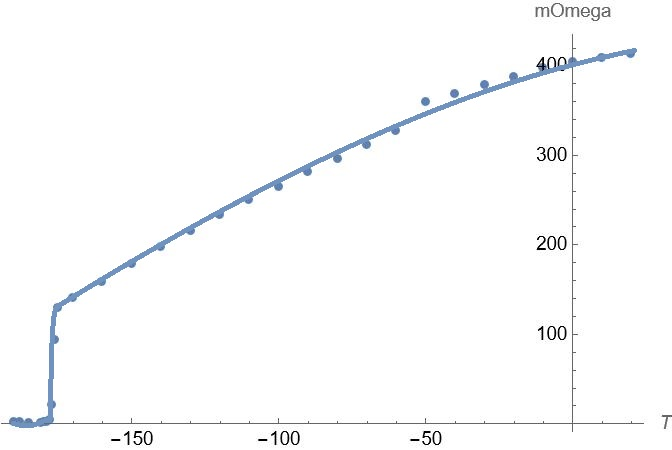
\includegraphics[width=0.8\textwidth]{img/1-1.jpg} %插入图片,[]中设置图片大小,{}中是图片文件名
    %         \caption{降温时电阻-温度曲线} %最终文档中希望显示的图片标题
    %         \label{降温RT} %用于文内引用的标签
    %     \end{minipage}
    %     \begin{minipage}[t]{0.48\linewidth}
    %         \centering %图片居中
    %         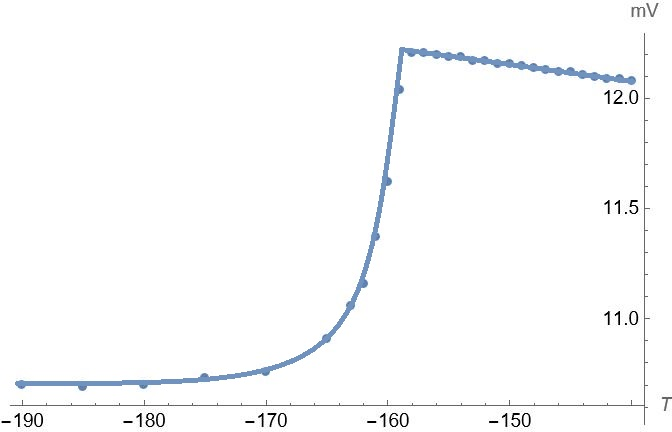
\includegraphics[width=0.8\textwidth]{img/1-2.jpg} %插入图片,[]中设置图片大小,{}中是图片文件名
    %         \caption{降温时感应电动势-温度曲线} %最终文档中希望显示的图片标题
    %         \label{降温UT} %用于文内引用的标签
    % \end{minipage}
    % \end{figure}

    \begin{figure}[H] %H为当前位置,!htb为忽略美学标准,htbp为浮动图形
        \centering %图片居中
        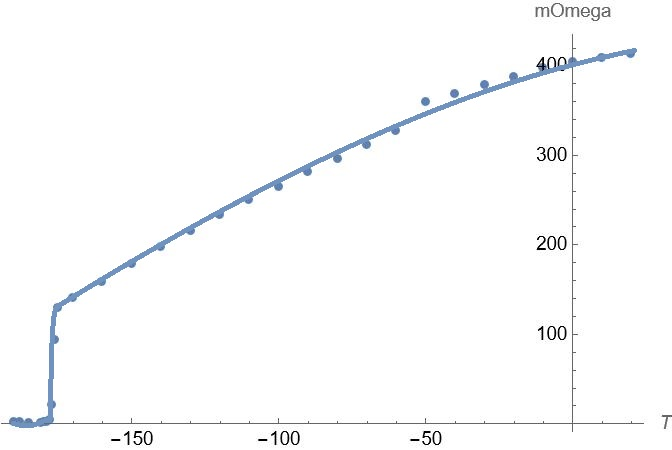
\includegraphics[width=0.5\textwidth]{img/1-1.jpg} %插入图片,[]中设置图片大小,{}中是图片文件名
        \caption{降温时电阻-温度曲线} %最终文档中希望显示的图片标题
        \label{降温RT} %用于文内引用的标签
    \begin{figure}[H] %H为当前位置,!htb为忽略美学标准,htbp为浮动图形
    \end{figure}
        \centering %图片居中
        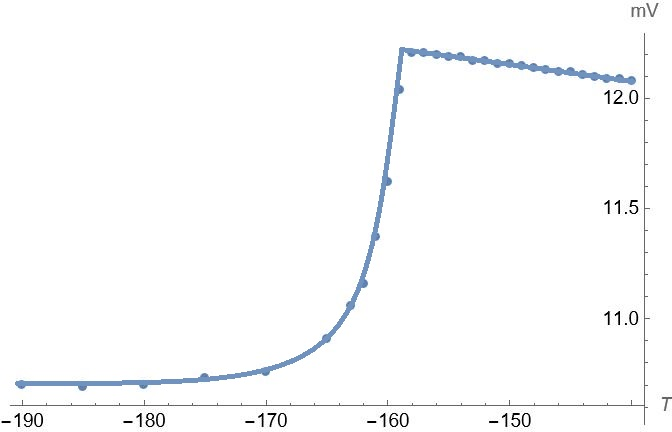
\includegraphics[width=0.5\textwidth]{img/1-2.jpg} %插入图片,[]中设置图片大小,{}中是图片文件名
        \caption{降温时感应电动势-温度曲线} %最终文档中希望显示的图片标题
        \label{降温UT} %用于文内引用的标签
    \end{figure}

    \subsubsection{升温}

    \begin{table}[H]
        \centering
        \begin{tabular}{|l|l|l|l|l|l|l|l|l|l|l|}
        \hline
            温度($^{\circ}$C) & -190 & -185 & -180 & -175 & -170 & -165 & -163 & -162 & -161 & -160 \\ \hline
            $R_{Sample}$(m$\Omega$) & 2 & 2 & 3 & 3 & 2 & 3 & 2 & 3 & 3 & 5 \\ \hline
            $V_B$(mV) & 10.70 & 10.69 & 10.70 & 10.73 & 10.76 & 10.91 & 11.06 & 11.16 & 11.37 & 11.62 \\ \hline
            \hline
            温度($^{\circ}$C) & -159 & -158 & -157 & -156 & -155 & -154 & -153 & -152 & -151 & -150 \\ \hline
            $R_{Sample}$(m$\Omega$) & 15 & 57 & 121 & 131 & 132 & 134 & 135 & 137 & 139 & 140 \\ \hline
            $V_B$(mV) & 12.04 & 12.21 & 12.21 & 12.20 & 12.19 & 12.19 & 12.17 & 12.17 & 12.16 & 12.16 \\ \hline
            \hline
            温度($^{\circ}$C) & -149 & -148 & -147 & -146 & -145 & -144 & -143 & -142 & -141 & -140 \\ \hline
            $R_{Sample}$(m$\Omega$) & 141 & 142 & 143 & 146 & 147 & 148 & 150 & 151 & 153 & 154 \\ \hline
            $V_B$(mV) & 12.15 & 12.14 & 12.13 & 12.12 & 12.12 & 12.11 & 12.10 & 12.09 & 12.09 & 12.08 \\ \hline
        \end{tabular}
        \caption{升温做图表格} %最终文档中希望显示的图片标题
        \label{升温做图表格} %用于文内引用的标签
    \end{table}

    % \begin{figure}[H] %H为当前位置,!htb为忽略美学标准,htbp为浮动图形
    %     \begin{minipage}[t]{0.48\linewidth}
    %         \centering %图片居中
    %         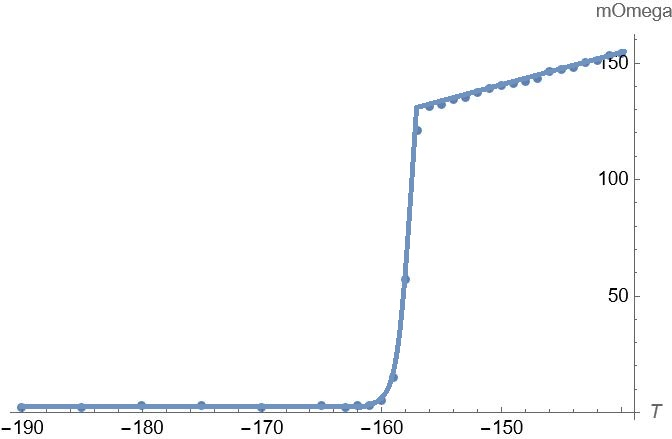
\includegraphics[width=0.8\textwidth]{img/2-1.jpg} %插入图片,[]中设置图片大小,{}中是图片文件名
    %         \caption{升温时电阻-温度曲线} %最终文档中希望显示的图片标题
    %         \label{升温RT} %用于文内引用的标签
    %     \end{minipage}
    %     \begin{minipage}[t]{0.48\linewidth}
    %         \centering %图片居中
    %         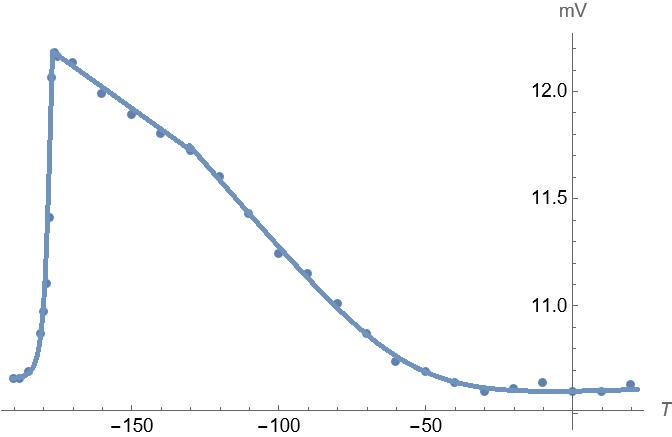
\includegraphics[width=0.8\textwidth]{img/2-2.jpg} %插入图片,[]中设置图片大小,{}中是图片文件名
    %         \caption{升温时感应电动势-温度曲线} %最终文档中希望显示的图片标题
    %         \label{升温UT} %用于文内引用的标签
    % \end{minipage}
    % \end{figure}

    \begin{figure}[H] %H为当前位置,!htb为忽略美学标准,htbp为浮动图形
        \centering %图片居中
        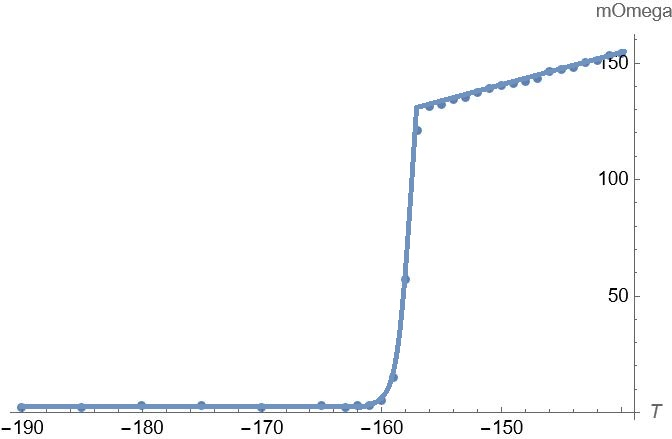
\includegraphics[width=0.5\textwidth]{img/2-1.jpg} %插入图片,[]中设置图片大小,{}中是图片文件名
        \caption{升温时电阻-温度曲线} %最终文档中希望显示的图片标题
        \label{升温RT} %用于文内引用的标签
    \end{figure}
    \begin{figure}[H] %H为当前位置,!htb为忽略美学标准,htbp为浮动图形
        \centering %图片居中
        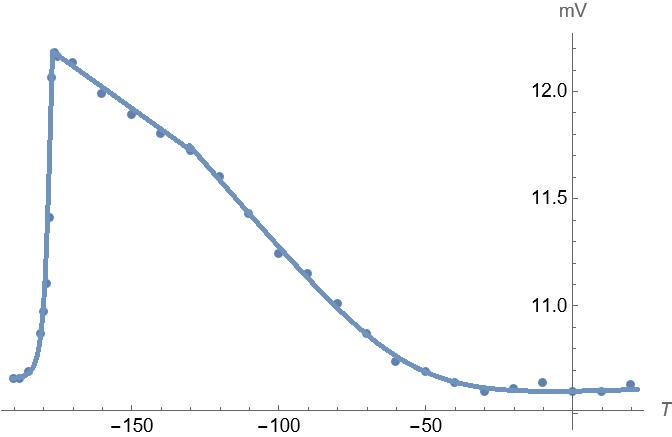
\includegraphics[width=0.5\textwidth]{img/2-2.jpg} %插入图片,[]中设置图片大小,{}中是图片文件名
        \caption{升温时感应电动势-温度曲线} %最终文档中希望显示的图片标题
        \label{升温UT} %用于文内引用的标签
    \end{figure}

    可以看出:电阻阻值和感应电动势在$-157\sim-161^{\circ}$C时产生了突变,故转变温度$T=-159^{\circ}$C,转变宽度$\Delta T=4^{\circ}$C

    \subsection{分析讨论}

    在降温的时候可以观察到样品电阻在$T=-178^{\circ}$C附近发生了突变,在升温的时候可以观察到
    样品电阻在$T=-159^{\circ}$C附近发生了突变,两次突变温度不同的原因可能是降温太快导致样品与温度计温度不相等,
    从而导致测量偏差。

\section{思考题}

    设想一个中空的超导圆管样品,转变温度为$T^{\circ}$C。在温度高于$T^{\circ}$C时,对圆管施加外磁场。
    而后将温度降低到转变温度$T^{\circ}$C以下。

    分析样品的磁感应强度和感应电流。撤掉外磁场后,样品的磁感应强度和感应电流如何变化:

    ~

    当温度低于临界温度(即转变温度$T_c$)时,超导材料会表现出零电阻和磁通排斥的特性。在这个温度范围内,超导圆管样品
    的磁感应强度为0,产生了感应电流以抵消样品内部的磁场

    撤掉外磁场后,由于超导现象,样品的磁感应强度仍然为0,但是会产生新的感应电流来维持样品内部磁场不变。

\newpage
\section{教师签字的原始实验数据}
    \begin{center}
        \begin{figure}[H] %H为当前位置,!htb为忽略美学标准,htbp为浮动图形
            \centering %图片居中
            \includegraphics[width=0.8\textwidth]{img/OriginalData1.jpg} %插入图片,[]中设置图片大小,{}中是图片文件名
            \caption{原始数据1} %最终文档中希望显示的图片标题
            \label{原始数据-1} %用于文内引用的标签
        \end{figure}
        \begin{figure}[H] %H为当前位置,!htb为忽略美学标准,htbp为浮动图形
            \centering %图片居中
            \includegraphics[width=0.8\textwidth]{img/OriginalData2.jpg} %插入图片,[]中设置图片大小,{}中是图片文件名
            \caption{原始数据2} %最终文档中希望显示的图片标题
            \label{原始数据-2} %用于文内引用的标签
        \end{figure}
    \end{center}
\end{document}